\section{Evaluation Scheme}
The metric used in the competition for evaluating the models is accuracy. Additionally, we assess the model using precision, recall and F1-score in our work. We define them formally in the following subsection.

\subsection{Definitions}
% \sdaltcomment{Is this section required??}
% \sdaltcomment{Prec/Rec are only for label 1...}
We use the following notations in the definition of the metrics.
\begin{itemize}
    \item \textbf{TP} (True Positive): Model predicts hate spreader and is actually hate spreader.
    \item \textbf{FP} (False Positive): Model predicts hate spreader but is actually not hate spreader.
    \item \textbf{FN} (False Negative): Model predicts not hate spreader but is actually hate spreader.
    \item \textbf{TN} (True Negative): Model predicts not hate spreader and is actually not hate spreader.
\end{itemize}

The metrics mentioned earlier can be defined as follows:
\begin{table}[htpb]
\centering
\begin{tabular}{lcl}
Accuracy & = & $\frac{TP + TN}{TP + FP + FN + TN}$ \\
~ & ~ & ~ \\
Precision & = & $\frac{TP}{TP + FP}$ \\
~ & ~ & ~ \\
Recall & = & $\frac{TP}{TP + FN}$ \\
~ & ~ & ~ \\
F1-score & = & $\frac{2 \times \text{Precision} \times
\text{Recall}}{\text{Precision}+\text{Recall}}$ \\
\end{tabular}
\end{table}

\section{Baselines}

\subsection{Term-frequency based representation}
\label{sec:results:tf-idf}

% Please add the following required packages to your document preamble:
% \usepackage{multirow}
\begin{table}[htpb]
\centering
\begin{tabular}{llrrrr}
\hline
\textbf{Representation} & \textbf{Classifier} & \multicolumn{1}{l}{\textbf{Accuracy}} & \multicolumn{1}{l}{\textbf{Precision}} & \multicolumn{1}{l}{\textbf{Recall}} & \multicolumn{1}{l}{\textbf{F1-score}} \\ \hline
\multirow{4}{*}{Count} & LR & 0.6500 & 0.6531 & 0.6400 & 0.6465 \\ 
 & SVM & 0.6600 & 0.6600 & 0.6600 & 0.6600 \\ 
 & NB & 0.6200 & 0.6111 & 0.6600 & 0.6346 \\ 
 & RF & 0.6500 & 0.6596 & 0.6200 & 0.6392 \\ \hline
\multirow{6}{*}{TF-IDF} & LR & \textbf{0.6900} & \textbf{0.6792} & 0.7200 & 0.6990 \\ 
 & SVM & \textbf{0.6900} & 0.6667 & 0.7600 & 0.7103 \\ 
 & NB & 0.6600 & 0.6026 & \textbf{0.9400} & \textbf{0.7344} \\ 
 & RF & 0.6100 & 0.6000 & 0.6600 & 0.6286 \\ 
 & XGB & 0.6000 & 0.6136 & 0.5400 & 0.5745 \\ 
 & LGBM & 0.6200 & 0.6034 & 0.7000 & 0.6481 \\ \hline
\end{tabular}
\caption{Performance of models trained with Term-frequency based representation (Section \ref{sec:models:tf-idf})}
\label{tab:results:performance-tf-based}
\end{table}
% \sdaltcomment{use acro in tables?}

From Table \ref{tab:results:performance-tf-based}, it can be observed that both \ac{TF-IDF}+\ac{LR} and \ac{TF-IDF}+\ac{SVM} have the best performance in terms of accuracy (69\%). However, \ac{TF-IDF}+\ac{NB} has the highest F1-score (73.43\%) among all the models. It also has a very high recall score of 94\%, i.e., it produces the least low false negatives. \ac{TF-IDF}+\ac{SVM} also has a competitive F1-score score of 71.02\%. Moreover, \ac{TF-IDF} vectorization performs better than simple Count vectorization. The best hyper-parameter values obtained after fine-tuning are listed in Table \ref{tab:best-hparams-tf-based-count-vect} (with Count Vectorizer) and Table \ref{tab:best-hparams-tf-based-tfidf-vect} (with \ac{TF-IDF} Vectorizer).


% % Please add the following required packages to your document preamble:
% % \usepackage{multirow}
% \begin{table}[htbp]
% \centering
% \begin{tabular}{llr}
% \hline
% \textbf{Model} & \textbf{Hyper-parameter} & \textbf{Values} \\ \hline
% \multirow{8}{*}{LR} & (Vectorizer) &  \\
%  & max\_df & 0.75 \\
%  & min\_df & 2 \\
%  & ngram\_range & (1, 2) \\
%  & (Classifier) &  \\
%  & C & 2 \\
%  & penalty & l1 \\
%  & solver & saga \\  \hline
% \multirow{7}{*}{SVM} & (Vectorizer) &  \\
%  & max\_df & 0.75 \\
%  & min\_df & 2 \\
%  & ngram\_range & (1, 2) \\
%  & (Classifier) &  \\
%  & C & 0.1 \\
%  & kernel & linear \\  \hline
% \multirow{6}{*}{NB} & (Vectorizer) &  \\
%  & max\_df & 1.0 \\
%  & min\_df & 2 \\
%  & ngram\_range & (1, 1) \\
%  & (Classifier) &  \\
%  & alpha & 0.005623413251903491 \\  \hline
% \multirow{11}{*}{RF} & (Vectorizer) &  \\
%  & max\_df & 1.0 \\
%  & min\_df & 5 \\
%  & ngram\_range & (1, 2) \\
%  & (Classifier) &  \\
%  & bootstrap & True \\
%  & max\_depth & 10 \\
%  & max\_features & auto \\
%  & min\_samples\_leaf & 2 \\
%  & n\_estimators & 100 \\
%  & oob\_score & True \\  \hline
% \end{tabular}
% \caption{Best hyper-parameter values for models trained with Term-frequency based representation (Section \ref{sec:models:tf-idf}) with Count Vectorizer \sdaltcomment{too long.. take transpose... move to Appendix?} }
% \label{tab:best-hparams-tf-based-count-vect}
% \end{table}

% % Please add the following required packages to your document preamble:
% % \usepackage{multirow}
% % \usepackage{longtable}
% % Note: It may be necessary to compile the document several times to get a multi-page table to line up properly
% \begin{longtable}[c]{llr}
% \hline
% \textbf{Model} & \textbf{Hyper-parameter} & \textbf{Values} \\ \hline
% \endhead
% %
% \multirow{8}{*}{LR} & (Vectorizer) &  \\
%  & max\_df & 1.0 \\
%  & min\_df & 10 \\
%  & ngram\_range & (1, 1) \\
%  & (Classifier) &  \\
%  & C & 10 \\
%  & penalty & l2 \\
%  & solver & saga \\ \hline
% \multirow{7}{*}{SVM} & (Vectorizer) &  \\
%  & max\_df & 0.75 \\
%  & min\_df & 10 \\
%  & ngram\_range & (1, 1) \\
%  & (Classifier) &  \\
%  & C & 2 \\
%  & kernel & rbf \\ \hline
% \multirow{6}{*}{NB} & (Vectorizer) &  \\
%  & max\_df & 0.75 \\
%  & min\_df & 10 \\
%  & ngram\_range & (1, 1) \\
%  & (Classifier) &  \\
%  & alpha & 3.1622776601683795 \\ \hline
% \multirow{11}{*}{RF} & (Vectorizer) &  \\
%  & max\_df & 0.75 \\
%  & min\_df & 5 \\
%  & ngram\_range & (1, 1) \\
%  & (Classifier) &  \\
%  & bootstrap & True \\
%  & max\_depth & None \\
%  & max\_features & auto \\
%  & min\_samples\_leaf & 1 \\
%  & n\_estimators & 200 \\
%  & oob\_score & True \\ \hline
% \multirow{10}{*}{XGB} & (Vectorizer) &  \\
%  & max\_df & 1.0 \\
%  & min\_df & 2 \\
%  & ngram\_range & (1, 2) \\
%  & (Classifier) &  \\
%  & colsample\_bytree & 0.6 \\
%  & eta & 0.05 \\
%  & max\_depth & 7 \\
%  & n\_estimators & 100 \\
%  & subsample & 0.8 \\ \hline
% \multirow{10}{*}{LGBM} & (Vectorizer) &  \\
%  & max\_df & 1.0 \\
%  & min\_df & 10 \\
%  & ngram\_range & (1, 1) \\
%  & (Classifier) &  \\
%  & boosting\_type & dart \\
%  & colsample\_bytree & 0.6 \\
%  & learning\_rate & 0.05 \\
%  & n\_estimators & 50 \\
%  & subsample & 0.6 \\ \hline
% \caption{Best hyper-parameter values for models trained with Term-frequency based representation (Section \ref{sec:models:tf-idf}) with \ac{TF-IDF} Vectorizer \sdaltcomment{fix alignment...} }
% \label{tab:best-hparams-tf-based-tfidf-vect}\\
% \end{longtable}



%%%%%%%%%%%%%%%%%%%% SET UP 1 %%%%%%%%%%%%%%%%%%%
\begin{landscape}
\vspace*{\fill}
% Please add the following required packages to your document preamble:
% \usepackage{multirow}
\begin{table}[htbp]
    \centering
    \begin{tabular}{|l|rrr|rrrrrr|}
    \hline
    \multirow{2}{*}{\textbf{Model}} & \multicolumn{9}{c|}{\textbf{Hyper-parameters/Values}} \\
    \cline{2-10}
    & \multicolumn{3}{c|}{\textbf{Vectorizer}} & \multicolumn{6}{c|}{\textbf{Classifier}} \\
    \hline
    \multirow{2}{*}{LR} & max\_df & min\_df & ngram\_range  &  &  &  & C & penalty & solver  \\
                        & 0.75    & 2       & (1, 2)        &  &  &  & 2 & l1      & saga  \\
    \hline
    \multirow{2}{*}{SVM} & max\_df  & min\_df & ngram\_range &  &  &  &  & C   & kernel  \\
                         & 0.75     & 2       & (1, 2)       &  &  &  &  & 0.1 & linear  \\
    \hline
    \multirow{2}{*}{NB}  & max\_df  & min\_df & ngram\_range &  &  &  &  \multicolumn{3}{r|}{alpha}  \\
                         & 1.0      & 2        & (1, 1)      &  &  &  &  \multicolumn{3}{r|}{0.005623413251903491} \\
    \hline
    \multirow{2}{*}{RF}  & max\_df & min\_df & ngram\_range & bootstrap & max\_depth & max\_features & min\_samples\_leaf & n\_estimators & oob\_score \\
                         & 1.0     & 5       & (1, 2)       & True      & 10         & auto          & 2                  & 100           & True \\
    \hline
    \end{tabular}
    \caption{Best hyper-parameter values for models trained with Term-frequency based representation (Section \ref{sec:models:tf-idf}) with Count Vectorizer}
    \label{tab:best-hparams-tf-based-count-vect}
\end{table}

% Please add the following required packages to your document preamble:
% \usepackage{multirow}
\begin{table}[!h]
    \centering
    \begin{tabular}{|l|rrr|rrrrrr|}
    \hline
    \multirow{2}{*}{\textbf{Model}} & \multicolumn{9}{c|}{\textbf{Hyper-parameters/Values}} \\
    \cline{2-10}
    & \multicolumn{3}{c|}{\textbf{Vectorizer}} & \multicolumn{6}{c|}{\textbf{Classifier}} \\
    \hline
    \multirow{2}{*}{LR} & max\_df & min\_df & ngram\_range  &  &  &  & C & penalty & solver  \\
                        & 1.0     & 10      & (1, 1)        &  &  &  & 10 & l2      & saga  \\
    \hline
    \multirow{2}{*}{SVM} & max\_df & min\_df & ngram\_range &  &  &  &  & C  & kernel  \\
                         & 0.75    & 10      & (1, 1)       &  &  &  &  & 2  & rbf  \\
    \hline
    \multirow{2}{*}{NB}  & max\_df  & min\_df & ngram\_range &  &  &  &  \multicolumn{3}{r|}{alpha}  \\
                         & 0.75     & 10      & (1, 1)      &  &  &  &  \multicolumn{3}{r|}{3.1622776601683795} \\
    \hline
    \multirow{2}{*}{RF}  & max\_df & min\_df & ngram\_range & bootstrap & max\_depth & max\_features & min\_samples\_leaf & n\_estimators & oob\_score \\
                         & 0.75    & 5       & (1, 1)       & True      & None       & auto          & 1                  & 200           & True       \\
    \hline
    \multirow{2}{*}{XGB}  & max\_df  & min\_df & ngram\_range &  \multicolumn{2}{r}{colsample\_bytree} & eta  & max\_depth & n\_estimators & subsample \\
                          & 1.0      & 2       & (1, 2)       & \multicolumn{2}{r}{0.6}               & 0.05 & 7          & 100           & 0.8 \\
    \hline
    \multirow{2}{*}{LGBM}  & max\_df & min\_df & ngram\_range &  \multicolumn{2}{r}{boosting\_type} & colsample\_bytree & learning\_rate & n\_estimators & subsample   \\
                           & 1.0     & 10      & (1, 1)       &  \multicolumn{2}{r}{dart}           & 0.6               & 0.05           & 50            & 0.6   \\
    \hline
    \end{tabular}
    % \caption{Best hyper-parameter values for models trained with Term-frequency based representation (Section \ref{sec:models:tf-idf}) with \ac{TF-IDF} Vectorizer}
    \caption[Best hyper-parameter values for models trained with Term-frequency based representation (Section \ref{sec:models:tf-idf}) with \texorpdfstring{TF-IDF}{TF-IDF} Vectorizer]{Best hyper-parameter values for models trained with Term-frequency based representation (Section \ref{sec:models:tf-idf}) with \ac{TF-IDF} Vectorizer}
    
    {Feature importance from trained \ac{XGB}, \ac{RF} and \ac{LGBM} models in Section \ref{sec:models:feat-based}}
    \label{tab:best-hparams-tf-based-tfidf-vect}
\end{table}

\vfill
\clearpage
\end{landscape}
%%%%%%%%%%%%%%%%%% END SETUP 1 %%%%%%%%%%%%%%%%%%%


\subsection{Features based representation}
\label{sec:results:feat-extr}

\begin{table}[htbp]
\centering
\begin{tabular}{lrrrr}
\hline
\textbf{Classifier} & \multicolumn{1}{l}{\textbf{Accuracy}} & \multicolumn{1}{l}{\textbf{Precision}} & \multicolumn{1}{l}{\textbf{Recall}} & \multicolumn{1}{l}{\textbf{F1-score}} \\ \hline
LR & 0.5800 & 0.5870 & 0.5400 & 0.5625 \\
SVM & 0.5200 & 0.5278 & 0.3800 & 0.4419 \\
NB & 0.5100 & 0.5116 & 0.4400 & 0.4731 \\
RF & 0.5800 & 0.5741 & 0.6200 & 0.5962 \\
XGB & \textbf{0.6200} & \textbf{0.6154} & \textbf{0.6400} & \textbf{0.6275} \\
LGBM & 0.5500 & 0.5455 & 0.6000 & 0.5714 \\ \hline
\end{tabular}
\caption{Performance of models trained with Features based representation (Section \ref{sec:models:feat-based})}
\label{tab:results:performance-feat-based}
\end{table}

From Table \ref{tab:results:performance-feat-based}, we can observe a significant performance gap with this approach compared to the models from Section \ref{sec:results:tf-idf}. \ac{XGB} performs the best among all the models in this setup. The best hyper-parameter values obtained after fine-tuning are listed in Table \ref{tab:best-hparams-feat-based}.


% Please add the following required packages to your document preamble:
% \usepackage{multirow}
\begin{table}[htbp]
\centering
\begin{tabular}{llr}
\hline
\textbf{Model} & \textbf{Hyper-parameter} & \textbf{Values} \\ \hline
\multirow{3}{*}{LR} & C & 0.1 \\
 & penalty & l1 \\
 & solver & liblinear \\
 \hline
\multirow{2}{*}{SVM} & C & 100 \\
 & kernel & rbf \\
 \hline
NB & alpha & 1e-05 \\
 \hline
\multirow{6}{*}{RF} & bootstrap & True \\
 & max\_depth & None \\
 & max\_features & auto \\
 & min\_samples\_leaf & 2 \\
 & n\_estimators & 20 \\
 & oob\_score & True \\
 \hline
\multirow{5}{*}{XGB} & colsample\_bytree & 0.6 \\
 & eta & 0.05 \\
 & max\_depth & 7 \\
 & n\_estimators & 100 \\
 & subsample & 0.8 \\
 \hline
\multirow{5}{*}{LGBM} & boosting\_type & dart \\
 & colsample\_bytree & 0.6 \\
 & learning\_rate & 0.05 \\
 & n\_estimators & 200 \\
 & subsample & 0.6 \\ \hline
\end{tabular}
\caption{Best hyper-parameter values for models trained with Features based representation (Section \ref{sec:models:feat-based})}
\label{tab:best-hparams-feat-based}
\end{table}

%% \sdaltcomment{xgboost gini??}
We plot the \eat{Gini }feature importance from the trained \ac{XGB}, \ac{RF} and \ac{LGBM} models in Figure \ref{fig:results:feat-imp}. The "negative sentiment" feature has the highest importance in all of these. This is a strong observation and can be linked to the fact that Hate Speech either consists of abusive or harmful words or indirectly implies them, thus high negative sentiment score. We plan to move towards developing new models making use of this observation and hence do not perform further (recursive) hyper-parameter tuning for the models in this setup.



\begin{figure}[htbp]
     \centering
     \begin{subfigure}[b]{\textwidth}
         \centering
         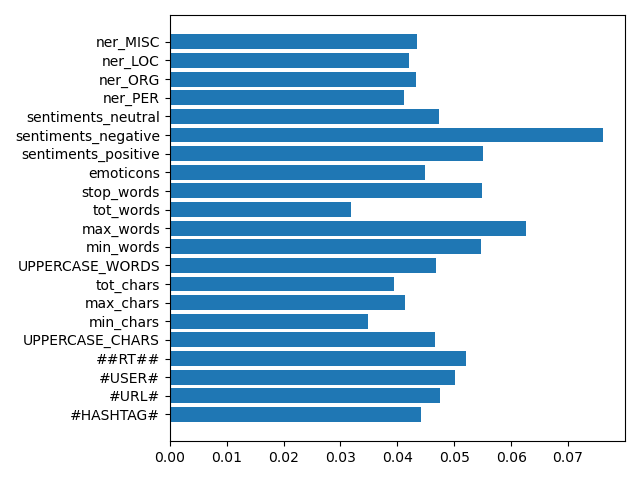
\includegraphics[width=0.75\textwidth]{assets/img/xgb_imp.png}
         \caption{\ac{XGB}}
         \label{fig:results:feat-imp::xgb}
         \vspace{0.6cm}
     \end{subfigure}
     \hfill
     \begin{subfigure}[b]{0.48\textwidth}
         \centering
         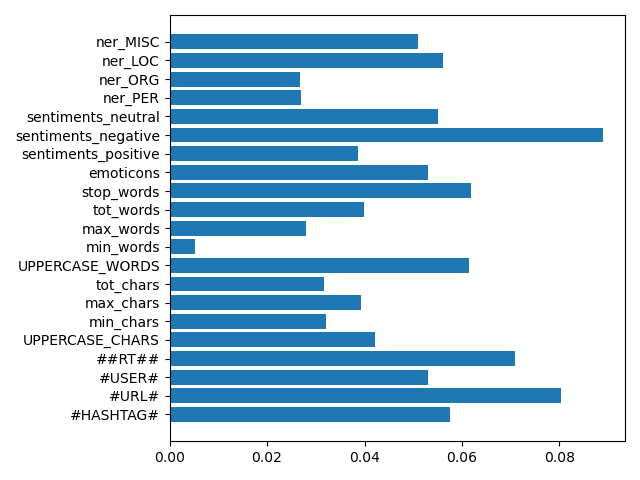
\includegraphics[width=\textwidth]{assets/img/rf_imp.png}
         \caption{\ac{RF}}
         \label{fig:results:feat-imp::rf}
     \end{subfigure}
     \hfill
     \begin{subfigure}[b]{0.48\textwidth}
         \centering
         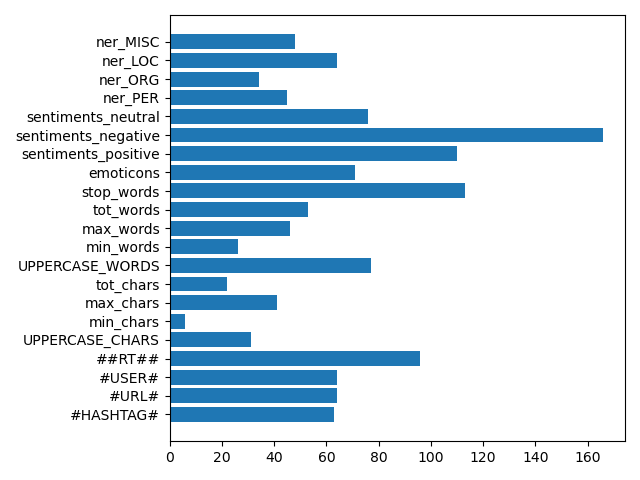
\includegraphics[width=\textwidth]{assets/img/lgb_imp.png}
         \caption{\ac{LGBM}}
         \label{fig:results:feat-imp::lgbm}
     \end{subfigure}
        \caption[Feature importance from trained \texorpdfstring{XGB}{XGB}, \texorpdfstring{RF}{RF} and \texorpdfstring{LGBM}{LGBM} models in Section \ref{sec:models:feat-based}]{Feature importance from trained \ac{XGB}, \ac{RF} and \ac{LGBM} models in Section \ref{sec:models:feat-based}}
        \label{fig:results:feat-imp}
\end{figure}
% https://tex.stackexchange.com/questions/551637/using-acronyms-in-toc

\newpage

\subsection{Word-embedding based representation}
\label{sec:results:word-emb}

% Please add the following required packages to your document preamble:
% \usepackage{multirow}
% \usepackage[table,xcdraw]{xcolor}
% If you use beamer only pass "xcolor=table" option, i.e. \documentclass[xcolor=table]{beamer}
\begin{table}[htbp]
\centering
\begin{tabular}{llrrrr}
\hline
\multicolumn{1}{l}{\textbf{Embedding}} &  & \multicolumn{1}{l}{} & \multicolumn{1}{l}{} & \multicolumn{1}{l}{} & \multicolumn{1}{l}{} \\
\multicolumn{1}{l}{\textbf{dimension}} & \multirow{-2}{*}{\textbf{Pooling}} & \multicolumn{1}{l}{\multirow{-2}{*}{\textbf{Accuracy}}} & \multicolumn{1}{l}{\multirow{-2}{*}{\textbf{Precision}}} & \multicolumn{1}{l}{\multirow{-2}{*}{\textbf{Recall}}} & \multicolumn{1}{l}{\multirow{-2}{*}{\textbf{F1-score}}} \\ \hline
 & Mean & 0.5200 & 0.5161 & 0.6400 & 0.5714 \\
 & Max. & 0.5200 & 0.5179 & 0.5800 & 0.5472 \\
 & Min. & 0.5500 & 0.5455 & 0.6000 & 0.5714 \\
\multirow{-4}{*}{25} & Abs. Max. & 0.5500 & 0.5556 & 0.5000 & 0.5263 \\ \hline
 & Mean & 0.4900 & 0.4923 & 0.6400 & 0.5565 \\
 & Max. & 0.4500 & 0.4444 & 0.4000 & 0.4211 \\
 & Min. & 0.5000 & 0.5000 & 0.5200 & 0.5098 \\
\multirow{-4}{*}{200} & Abs. Max. & 0.5100 & 0.5091 & 0.5600 & 0.5333 \\ \hline
\end{tabular}
\caption{Performance of models trained with Word-embedding based representation (Section \ref{sec:models:word-emb-based})}
\label{tab:results:performance-word-emb-based}
\end{table}


From Table \ref{tab:results:performance-word-emb-based}, we can observe that the models' performances are worse than the previous two setups. The fact that the training set is small (only 200 examples in training set) could be one of the reasons for not being able to train robust deep learning models from scratch.

